\documentclass{beamer}


\usepackage{graphicx} % Required for including images
\usepackage[utf8]{inputenc} % Required for inputting international characters
\usepackage{bookmark} % Add the bookmark package to handle changed files
\usepackage{booktabs}
\usetheme{CambridgeUS}
\usefonttheme{serif}
\usepackage{opensans}
\usepackage{amsmath}
\usepackage{amssymb}
\usepackage{amsfonts}
\usepackage{amsthm}





\title{The Discovery of an  Algebraic structure}
\subtitle{CSMI 2024}
\author[ASSIGBE Komi. RAHOUTI Chahid.]{ASSIGBE Komi \and  RAHOUTI Chahid}
\institute[]{University of Strasbourg \\ \smallskip} 


\date[\today]{Mathematics and applications \\ \today} 
% Presentation date or conference/meeting name, 
% the optional parameter can contain a shortened version to appear on the bottom 
% of every slide, while the required parameter value is output to the title slide
%----------------------------------------------------------------------------------------
%----------------------------------------------------------------------------------------
%   TITLE SLIDE
%----------------------------------------------------------------------------------------

\begin{document}

    \begin{frame}
        \titlepage% Print the title page as the first slide
    \end{frame}
    %----------------------------------------------------------------------------------------
    %   TABLE OF CONTENTS SLIDE
    %----------------------------------------------------------------------------------------


    \begin{frame}
        \frametitle{Table of contents}
        \tableofcontents
    \end{frame}
    % ---------------------------------------------------------------------
    %   PRESENTATION BODY SLIDES
    %----------------------------------------------------------------------------------------

    \section{Introduction}
    %------------------------------------------------
    \subsection{Definition}
    \begin{frame}
        \frametitle{Definition}
        What is an Algebraic structure? An algebraic structure consists of a nonempty set A (called the underlying set, carrier set or domain), a collection of operations on A (typically binary operations such as addition and multiplication), and a finite set of identities, known as axioms, that these operations must satisfy.
        Among the multiples algebraic structures, we can name:
        \begin{itemize}
            \item Group
            \item Ring
            \item Field
            \item Vector space
            \item .....
        \end{itemize}
    \end{frame}
    %------------------------------------------------

    %---------------------------------------------------------------------------------
    \section{Objectives}
    \begin{frame}
        \frametitle{The Main Objective}
        Our Main objective consist,  if we are giving a set of data in V, and those data is defined on a regular surface or variety, and we want to know if it is possible to detect a certain algebraic structure using Neural Networks Learning.
    \end{frame}


    \subsection{First sub objective} 
    \begin{frame}
        \frametitle{Implementing a Loss function based on the axioms of a
        algebraic structure}
        Let's take an example of a group structure.
        let consider a surface $M \in \mathbb{R}^{n \times n}$
        Like, 
        M = 
        $
        \begin{bmatrix}
            \vdots & \vdots & \vdots &\vdots \\
            x_{1} & x_{2} & \cdots & x_{n} \\
            \vdots & \vdots & \vdots &\vdots \\
        \end{bmatrix}
        $
        with $ x_{i} \in \mathbb{R}^{d}$
        The question is if we consider M as a group structure, it is possible to find a binary operation ($\circ$) on M such that M is a group.
        \begin{enumerate}
            $\exists e \in M, \forall x \in M, e \circ x = x \circ e = x$
            $\forall x,y \in M, x \circ y = y \circ x$
            $\forall x,y,z \in M, (x \circ y) \circ z = x \circ (y \circ z)$
            $\forall x \in M, \exists -x \in M, x \circ (-x) = (-x) \circ x=e$
        with x_{i} $\in \mathbb{R}^{d}$
        \end{enumerate}
        The question is if we consider M as a group structure, it is possible to find a binary operation ($\circ$) on M such that M is a group.
        
    \end{frame}
    %---------------------------------------------------------------------------------
    \subsection{Second sub objective}
    \begin{frame}

        \frametitle{Find a binary operation on V and a function f }



        Let's take an example of a group structure.
        let consider a set of points  $ V $ and let  $ f: R \rightarrow V $ a one-to-one
        function from $R$ into a codomain $V$. We define the vector addition by

        $$ x \oplus y = f(f^{-1}(x) + f^{-1}(y)) $$
        $$ \alpha \odot x = f(f^{-1}(x) * \alpha) $$


        The question is if we consider $V$ as a Vector Space, it is possible to find a binary operation ($\oplus$) and ($\odot$) on $V$ such that $V$ is a Vector Space.
        
    \end{frame}
    %---------------------------------------------------------------------------------


    \section{Examples}
    \begin{frame}
        \frametitle{Examples}
        \begin{itemize}
            \item Let f be a function from $R$ to $Vect{e_1}$ such that $f(x) = x.e_1$.
            we have $f^{-1}(x) = \lambda$.
                we take x and y in $vect{e_1}$, we have \\
                $x\oplus y = f(f^{-1}(x) + f^{-1}(y)) = x + y$ \\
                $\alpha \odot x = f(f^{-1}(x) * \alpha) = \alpha x$
                \item Let $\beta$ be any positive real number and let $f: \mathbb{R} \rightarrow \mathbb{R}^{+}$be defined by $f(x)=(1 / \beta) e^x$. Then $f$ is a one-to-one function from $\mathbb{R}$ onto the set of positive real numbers, and $f^{-1}(x)=\ln (\beta x)$ for $x>0$. we would define vector addition and scalar multiplication by
                $$ 
                x \oplus y=\frac{1}{\beta} e^{\ln (\beta x)+\ln (\beta y)}=\beta x y
                $$
                $$
                \alpha \odot x=\frac{1}{\beta} e^{\alpha \ln (\beta x)}=\beta^{\alpha-1} x^\alpha.
                $$
            \end{itemize}
    \end{frame}


        \section{Tools}
        \begin{frame}{Tools}
            For the implementation of this project, we are going to use :
            \begin{itemize}
                \item Python
                \item Pytorch
                \item Using Neural Networks learning by transforming the axioms of
                an Algebraic structure into a loss to minimize.
                \item using slack to communicate and share Idea
                \item Using Git to share code and work togeether
            \end{itemize}
        \end{frame}

    \section{Roadmap}
    \begin{frame}
        \begin{center}
            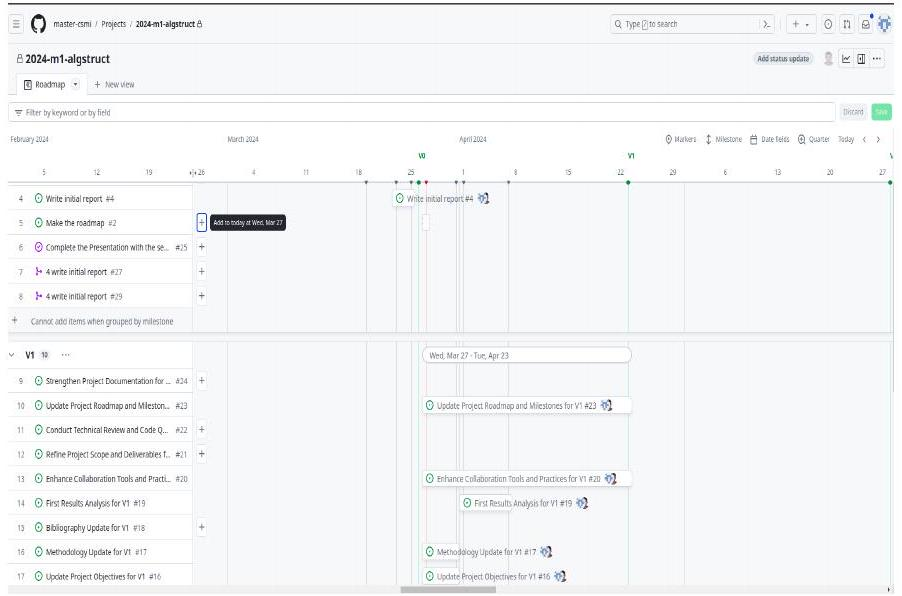
\includegraphics[width=9cm, height=6cm]{roadmap.png}
            %\caption{Roadmap}
        \end{center}
    \end{frame}
            




        
    \section{Application}
    \begin{frame}
        \frametitle{Application}
        Many differential equations encountered 
        in solving have parametric solutions.
        Thus, to find the solution for each 
        parameter, this often requires 
        numerous calculations. To optimize 
        computation and storage times, we 
        define an algebraic structure 
        whereby, if we compute the solution 
        for parameters $\lambda_1$ and $ \lambda_2 $,
        we can deduce $\lambda_3$
    \end{frame}

    
    
\end{document} 

